\chapter{Analysis}
Template article citation\cite{articleTemplate}\\
Template online citation\cite{onlineTemplate}\\
Template book citation with page range\cite[p.~442-444]{interactionDesign}

\section{Analysis Intro}
In this analysis, the focus will be on the investigation of the current issues with the fundamentals of musical education in elementary schools.\\
\\
Furthermore, current tools and technological inventions will be investigated to incorporate the same aspects to a final prototype.

\section{The impact of musical education}
Several studies have shown that different types of musical engagement in a variety of ways over a lifespan has an impact on several aspects of personal development. As concluded in the article "The power of music: Its impact on the intellectual, social and personal development of children and young people":\\

\begin{quote}
	\textit{"This overview provides a strong case for the benefits of active engagement with music throughout the lifespan"}\cite{powerOfMusic}\label{quote:powerOfMusic}.\\
\end{quote}

Linguistic abilities and musical training seem to be linked as shared brain mechanisms are used to process music and language. Precision in the perception of speech related contrasts in pitch patterns and other distinctive speech elements have been reported to be associated with musical ability\cite{languageSkills}.

A study focused on literary skills showed that a group of second grade students(n = 47) taking piano lessons over a 3-year period had significantly better vocabulary and verbal abilities than a group of control students(n = 57) that did not receive music lessons\cite{vocabularySkills}.

Some aspects of mathematical skills have also shown to be improved by musical training. For example the sub-division process required to read and play from music scores in order to play keep a rhythm\cite{powerOfMusic}.

Other abilities have also been reported to be affected by musical training such as creativity, social and personal development, physical development, health and wellbeing\cite{powerOfMusic}.


\section{Problem Area}

\begin{itemize}
	\item[-] Based on interviews and observations done with teachers and students
	\item[-] Issues in a musical classroom
	\item[-] Current tools, methods and the issues which is current utilizing these resources
	\item[-] Possible investigations done beforehand and their results	
\end{itemize}

\section{Target Group}

\begin{itemize}
	\item[-] Elementary school children (Grade 1,2,3,4,5,6)
	\item[-] Potentially the teachers as a sub target group?\todo{Maybe other way around?}
\end{itemize}


\section{Interactivity of music learning}
	When trying to understand music in an interactive sense, one might look at another medium that incorporates interactivity: video games. In particular, one could look at interactive video games that focuses around music playing or teaching.
	
	The role of music education can be defined as:
	\begin{quote}
		\centering
		\textit{"Teaching children to love music"}\cite[p.~94]{interactiveMusicVideoGames}.\\
	\end{quote}
	shit
	
	\begin{quote}
		\textit{Other key factors in motivation theory that can be identified within good video games include curiosity and a sense of autonomy or control over the learning that is occurring}\cite[p.~92]{interactiveMusicVideoGames}.\\
	\end{quote}
	
	\cite{constructivism}

\section{State of the art}
	\subsection{Guitar hero}
		\begin{figure}[H]
			\centering
			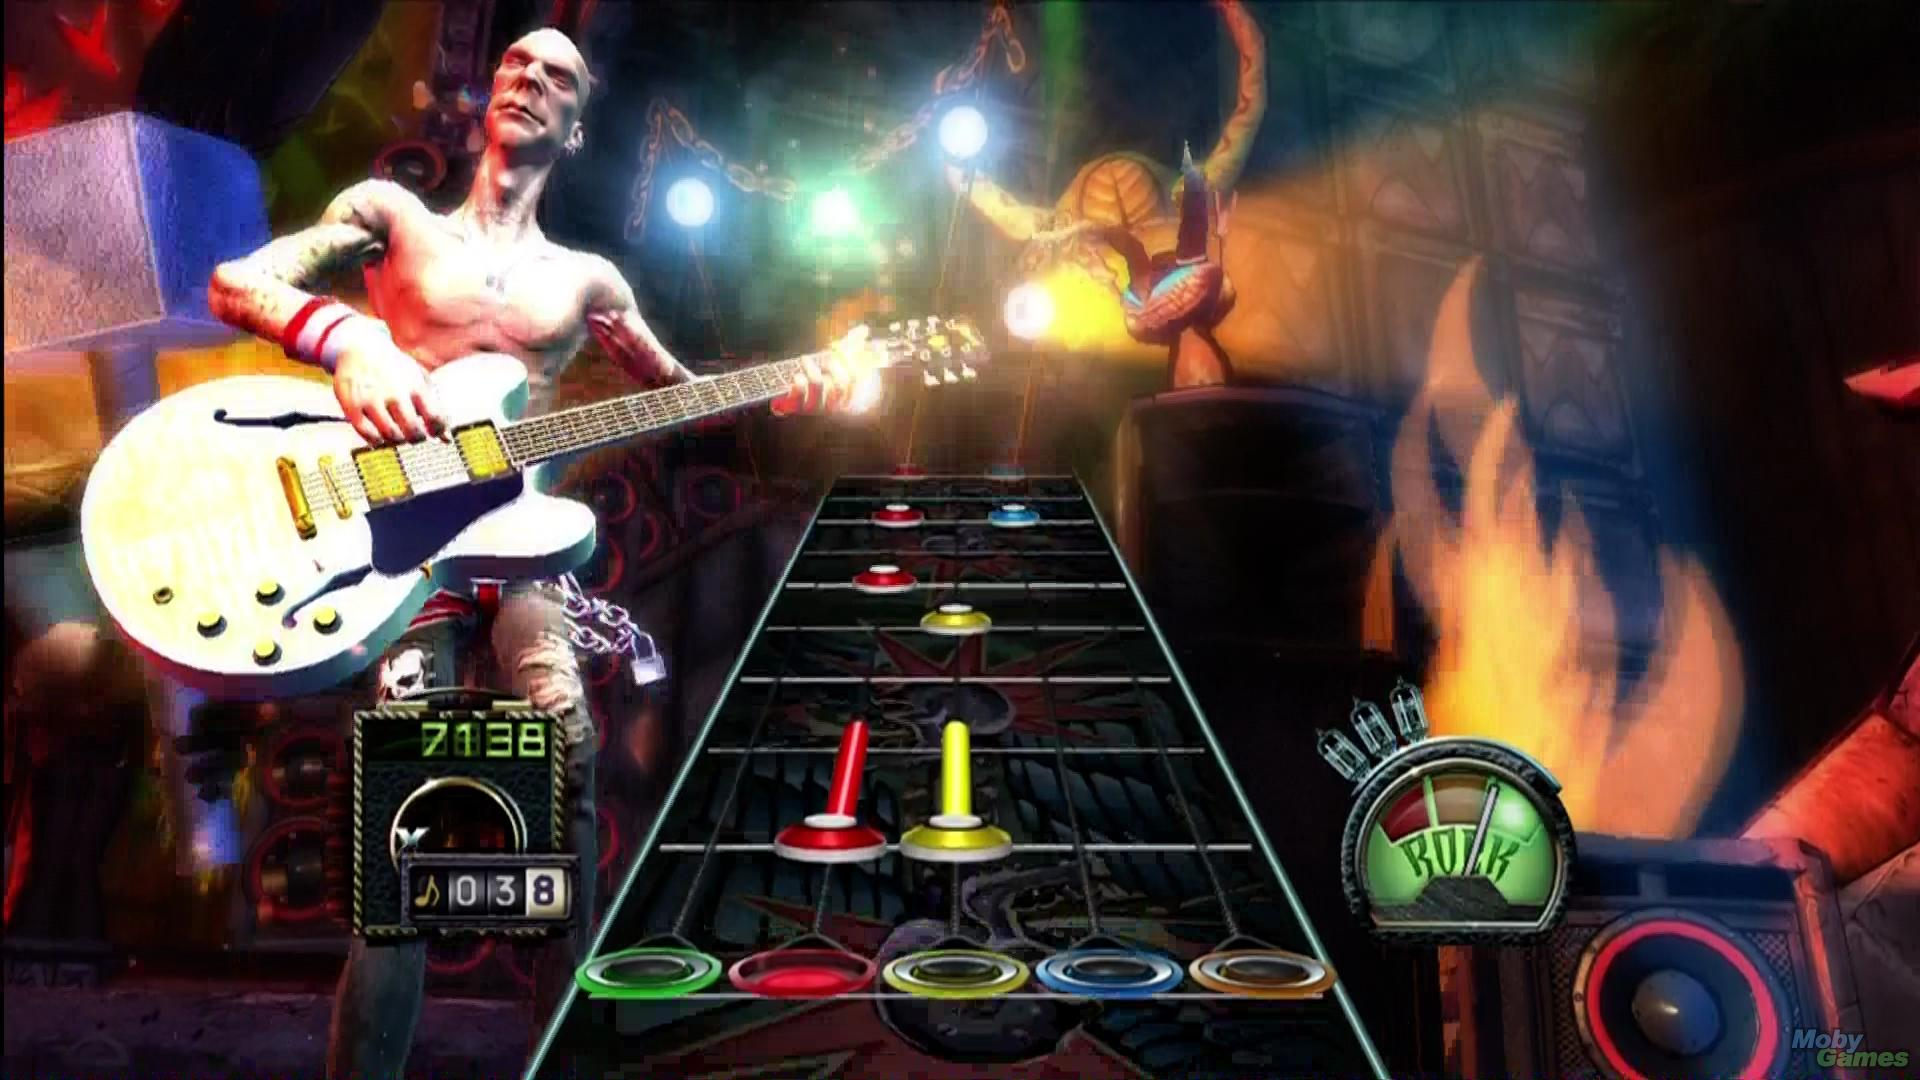
\includegraphics[width=0.7\linewidth]{figure/Analysis/guitarhero}
			\label{fig:guitarhero}
			\caption{Interactive music video game guitar hero.}
		\end{figure}
	\subsection{Noteput}
		German table where you physically put notes on it, and press play button to play notes, hopefully learning note and sheet theory.
	\subsection{Dato duo}
		Two person synthesizer for kids, to play around with, no apparent learning outcome, but seems fun to play around with.
		\begin{figure}[H]
			\centering
			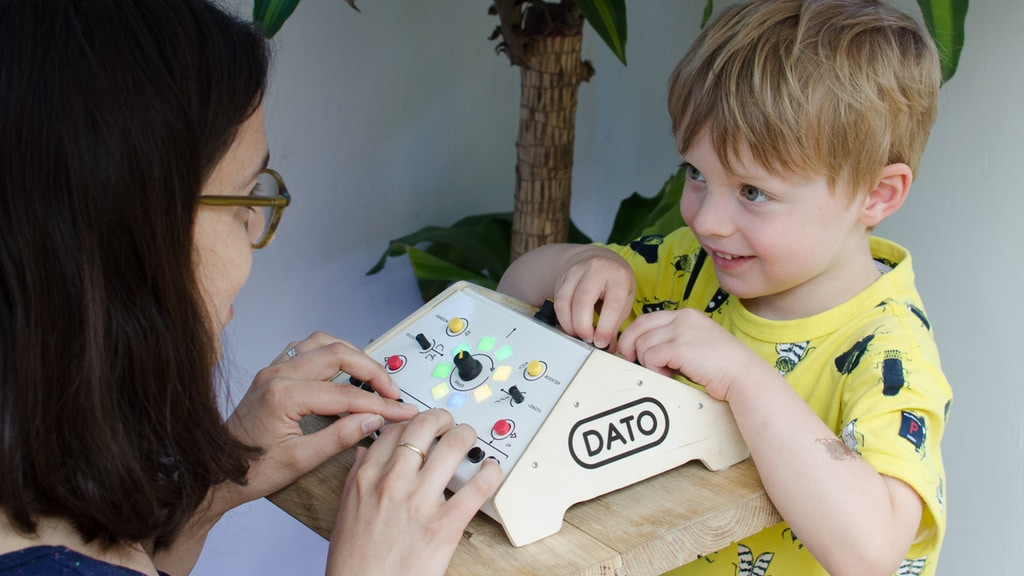
\includegraphics[width=0.7\linewidth]{figure/Analysis/datoduo}
			\label{fig:datoduo}
			\caption{Dato duo synthesizer}
		\end{figure}
	\subsection{Soundstage}
		VR application by Google, where you compose and play music in virtual reality. You can synthesize, plug things into other things, and create entire scores in this virtual reality playground.
		
	\subsection{V-Beat}
		The v-beat drumsticks are, for all its intents and purposes, simply air drumming.
		\begin{figure}[H]
			\centering
			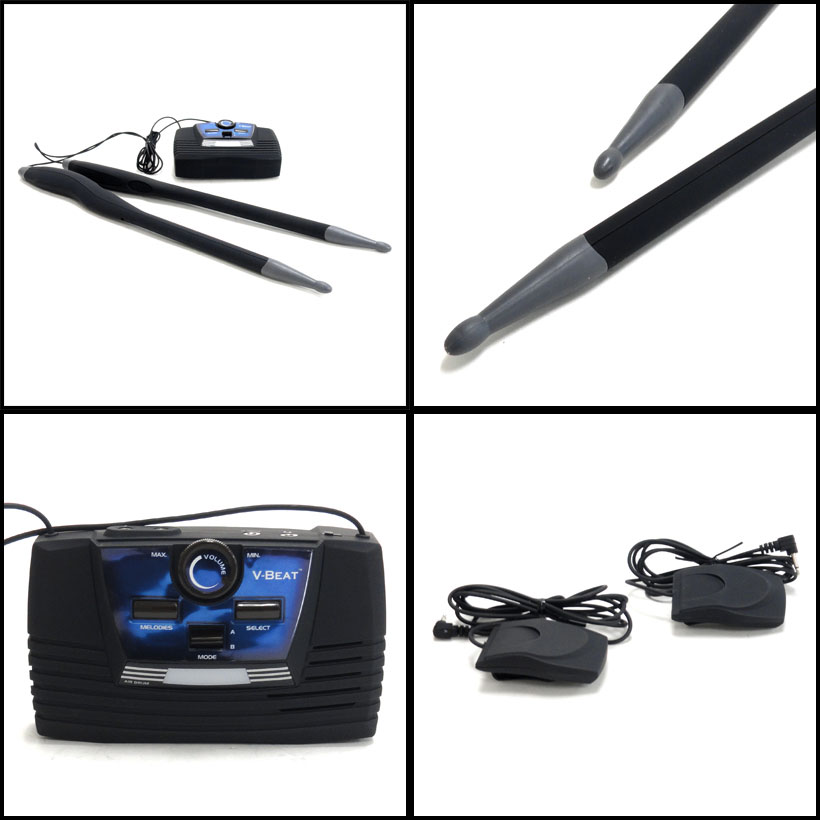
\includegraphics[width=0.5\linewidth]{figure/Analysis/vbeat}
			\label{fig:vbeat}
			\caption{Vbeat drumsticks}
		\end{figure}
		
	\subsection{MI Guitar}
		\begin{figure}[H]
			\centering
			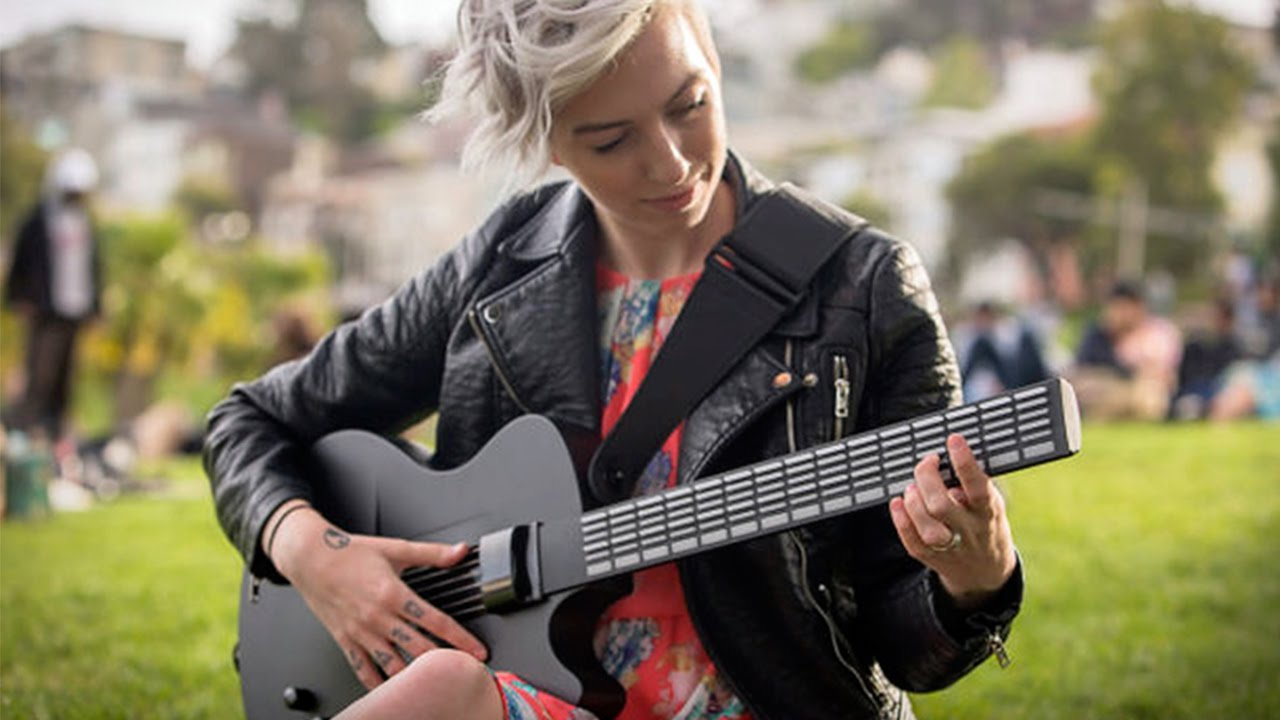
\includegraphics[width=0.8\linewidth]{figure/Analysis/miguitar}
			\label{fig:miguitar}
			\caption{MI guitar to teach guitar play}
		\end{figure}
	
	\subsection{Yousician}
		\begin{figure}[H]
			\centering
			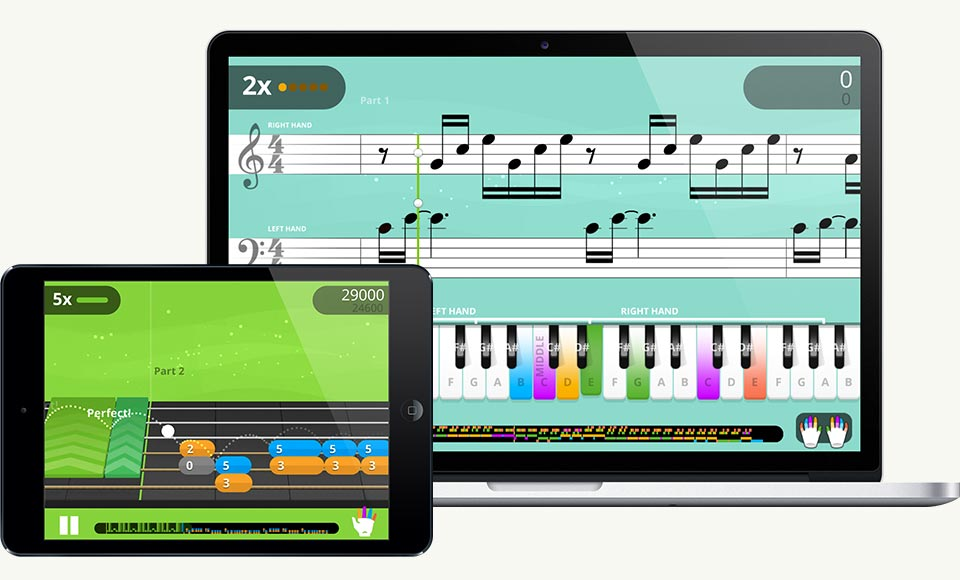
\includegraphics[width=0.8\linewidth]{figure/Analysis/yousician.jpg}
			\label{fig:yousician}
			\caption{Yousician}
		\end{figure}
	
	\subsection{Chrome Music Lab}
		\begin{figure}[H]
			\centering
			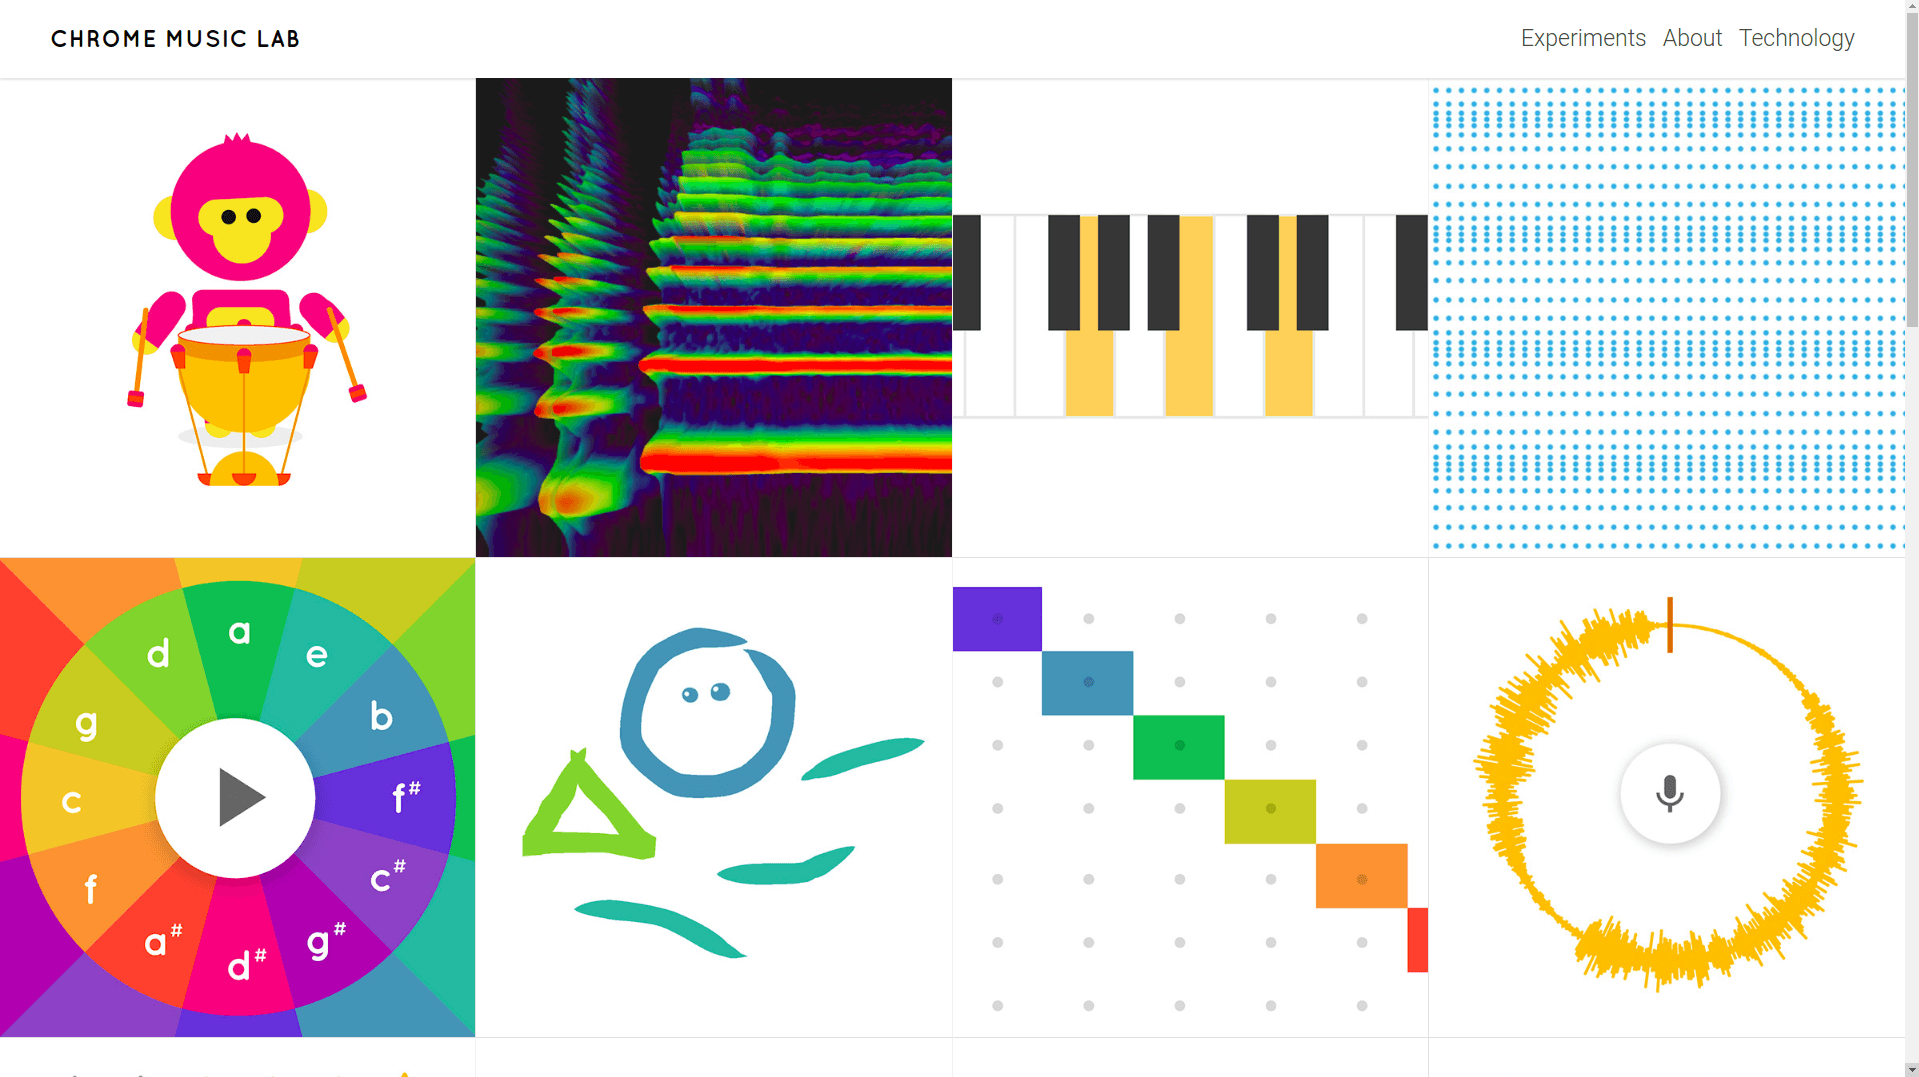
\includegraphics[width=0.8\linewidth]{figure/Analysis/chromeMusicLab.png}
			\label{fig:chromeMusicLab}
			\caption{Chrome Music Lab}
		\end{figure}

		